\documentclass[UTF8]{ctexart}
\usepackage{ctex}
\usepackage{graphicx}
\usepackage{color}
\usepackage{xcolor}
\usepackage{listings}
\usepackage{float}
\usepackage{amsmath}
\usepackage{tikz}
\usepackage{pgfplots}
\usepackage{fancyhdr}
\usepackage{mdframed}
\usepackage{caption}
\usepackage{ booktabs}
\usepackage{makecell}
\usepackage{amsthm}
\usepackage{hyperref }
\usepackage{ pgffor }
\usepackage{caption}
\usepackage{subcaption}
\usepackage{fancyhdr}
\usepackage{graphicx}
\usepackage{geometry} % 页面边距设置
\geometry{left=2.5cm, right=2.5cm, top=2.5cm, bottom=2.5cm}


%================================================================================================================%
\begin{document}

% 插入图片,调整宽度为页面宽度
\begin{center}
    
\includegraphics[width=\textwidth]{o} % 替换为您的图片文件名
\end{center}

% 定义标题
\begin{center}
    \huge\textbf{第一周实验报告}
\end{center}

% 定义作者
\begin{center}
    \huge\textbf{於佳杰}
\end{center}
% 以下内容将从下一页开始
\newpage
\title{第一周实验报告}
\author{於佳杰}
\date{2024 年 8 月 27 日}
\maketitle
\pagenumbering{arabic}
\tableofcontents
\newpage


\pagenumbering{arabic}

\pagestyle{fancy}
\fancyhf{}
\renewcommand{\headrulewidth}{1pt}
\renewcommand{\footrulewidth}{1pt}
\fancyhead[L]{
\includegraphics[width=1.5cm]{okkl}} % 确保图片路径正确
\fancyhead[C]{\rightmark}
\fancyfoot[C]{\thepage}
\fancyhead[R]{\thepage}







% 1实验目的================================================================================================%

\section{实验目的}
{\color{red}掌握LaTex和git的应用}
% 2实例展示================================================================================================%
\section{实例展示}

%1.1LaTex=========================================================================%
  \subsection{LaTex}
  {\color{blue}LaTex命令展示}



%1.1.1列表==================================================%
\subsubsection{列表}

\begin{enumerate}
  \item 有序列表(enumerate)
   \begin{itemize}
      \item 命令展示
\begin{lstlisting}
  \begin{enumerate}
   \item First thing

   \item Second thing
     \begin{itemize}
        \item A sub-thing

        \item Another sub-thing
     \end{itemize}

   \item Third thing

  \end{enumerate}
\end{lstlisting}
      \item 效果展示
\begin{enumerate}
  \item First thing

  \item Second thing
    \begin{itemize}
      \item A sub-thing

      \item Another sub-thing
    \end{itemize}

  \item Third thing
\end{enumerate}
   \end{itemize}

  \item 无序列表(itemize)
     \begin{itemize}
      \item 命令展示

\begin{lstlisting}
\begin{itemize}
   \item[@] First hello
   \item[@] first hello
   \item[@] first hello0
   \item[*] Second bye
   \item[*] second bye
   \item[*] second byee
    \begin{itemize}
   \item[cat] A sub-thing
   \item[cat] B sub-thing
   \item[cat] C sub-thing
   \item[Plants] Another sub-thing
   \item[Plants] Another sub-thing
   \item[Plants] Another sub-thing
    \end{itemize}
   \item[My] Third thing
   \item[My] Third cat
   \item[My] Third dog
\end{itemize}

\end{lstlisting}

      \item 效果展示
\begin{itemize}
   \item[@] First hello
   \item[@] first hello
   \item[@] first hello0
   \item[*] Second bye
   \item[*] second bye
   \item[*] second byee
    \begin{itemize}
   \item[cat] A sub-thing
   \item[cat] B sub-thing
   \item[cat] C sub-thing
   \item[Plants] Another sub-thing
   \item[Plants] Another sub-thing
   \item[Plants] Another sub-thing
    \end{itemize}
   \item[My] Third thing
   \item[My] Third cat
   \item[My] Third dog
\end{itemize}

\end{itemize}
\end{enumerate}

%1.1.2表格==================================================%
\subsubsection{表格}

\begin{enumerate}
  \item 普通表格(tabular)
    \begin{itemize}
      \item 命令展示

\begin{lstlisting}
\begin{table}
\center

\begin{tabular}{|c| c| c|}
\hline
okk & okk & okk\\
\hline\hline
okk & okk & okk\\
\hline
okk & okk & okk\\
\hline
\end{tabular}
\end {table}

\begin{table}
\center

\begin{tabular}{| l | r | r | r |}
\hline
City & \multicolumn{3}{c|}{Year} \\
\hline
& 2006 & 2007 & 2008 \\
\hline
London & 45789 & 46551 & 51298 \\
Berlin & 34549 & 32543 & 29870 \\
Paris & 49835 & 51009 & 51970 \\
\hline
\end{tabular}
\end {table}

\end{lstlisting}
      \item 效果展示


\begin{table}[H]
\center
\caption{假装是个表}
\begin{tabular}{|c| c| c|}
\hline
okk & okk & okk\\
\hline\hline
okk & okk & okk\\
\hline
okk & okk & okk\\
\hline
\end{tabular}
\end {table}


\begin{table}[H]
\center
\caption{假装是个表}
\begin{tabular}{| l | r | r | r |}
\hline
City & \multicolumn{3}{c|}{Year} \\
\hline
& 2006 & 2007 & 2008 \\
\hline
London & 45789 & 46551 & 51298 \\
Berlin & 34549 & 32543 & 29870 \\
Paris & 49835 & 51009 & 51970 \\
\hline
\end{tabular}
\end {table}

 \end{itemize}
\end{enumerate}




%1.1.3图表==================================================%
\subsubsection{图片}
\begin{enumerate}
  \item 图片(figure)
   \begin{itemize}
      \item 命令展示
\begin{lstlisting}
\begin{figure}[H]
  \centering
\includegraphics[width=1\textwidth]{myimage}
  \caption{Here is my image}
  \label{image-myimage}
\end{figure
\end{lstlisting}
\item 效果展示
\begin{figure}[H]
  \centering
  
\includegraphics[width=1\textwidth]{good}
  \caption{Here is my image}
  \label{image-myimage}
\end{figure}
\end{itemize}
\end{enumerate}









%1.1.4基本数学公式==================================================%

\subsubsection{基本数学公式}
\begin{enumerate}
  \item 基本数学公式
   \begin{itemize}
      \item 命令展示
\begin{lstlisting}
\begin{align}
    \frac{d}{d x}\int_{0}^{\infty} f(s) \, d s &= f(x)   \\
    f(x) &= \sum_{i=0}^{\infty}\frac{f^{(i)}(0)}{i!} x^{i}   \\
    x &= \sqrt{\frac{x_{i}}{z} y} 
\end{align}

\end{lstlisting}
\item 效果展示
\begin{align}
    \frac{d}{d x}\int_{0}^{\infty} f(s) \, d s &= f(x) \\
    f(x) &= \sum_{i=0}^{\infty}\frac{f^{(i)}(0)}{i!} x^{i}  \\
    x &= \sqrt{\frac{x_{i}}{z} y} &
\end{align}

\end{itemize}
\end{enumerate}

%1.1.5画图==================================================%
\subsubsection{画简单图形}
\begin{enumerate}
  \item 画三角形
   \begin{itemize}
      \item 命令展示
\begin{lstlisting}
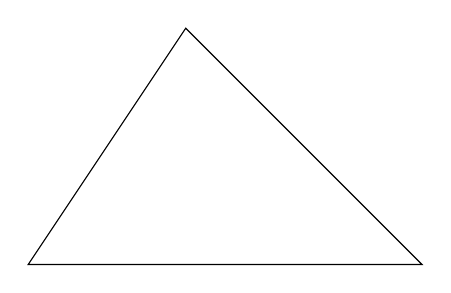
\begin{tikzpicture}
  \draw (0,0) -- (2,3) -- (5,0) -- cycle;
\end{tikzpicture}
\end{lstlisting}
\item 效果展示
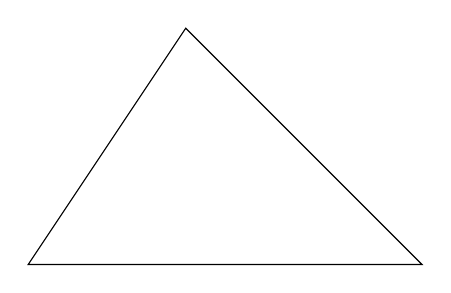
\begin{tikzpicture}
  \draw (0,0) -- (2,3) -- (5,0) -- cycle;
\end{tikzpicture}
\end{itemize}
\end{enumerate}


%1.1.6画函数图像==================================================%

\subsubsection{画函数图像}
\begin{enumerate}
  \item 绘制y=x*x函数图像
   \begin{itemize}
      \item 命令展示
\begin{lstlisting}
\begin{table}[H]
\centering
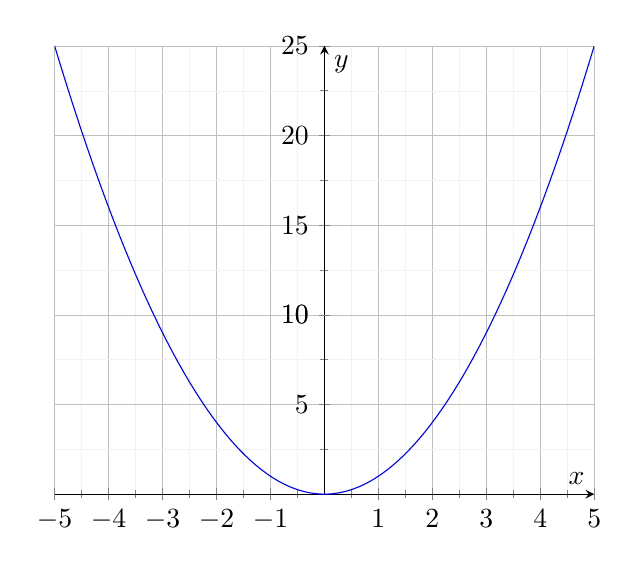
\begin{tikzpicture}
  \begin{axis}[
      xmin=-5, xmax=5,
      ymin=0, ymax=25,
      axis lines=middle,
      xlabel={$x$},
      ylabel={$y$},
      xtick={-5,-4,...,5},
      ytick={0,5,...,25},
      extra y ticks={10},
      grid=both,
      grid style={line width=.1pt, draw=gray!10},
      major grid style={line width=.2pt,draw=gray!50},
      minor tick num=1 
    ]
    \addplot[
      domain=-5:5,
      samples=100,
      color=blue, 
      ]
      {x^2};
  \end{axis}
\end{tikzpicture}
\end{table}
\end{lstlisting}
\item 效果展示
\begin{table}[H]
\centering
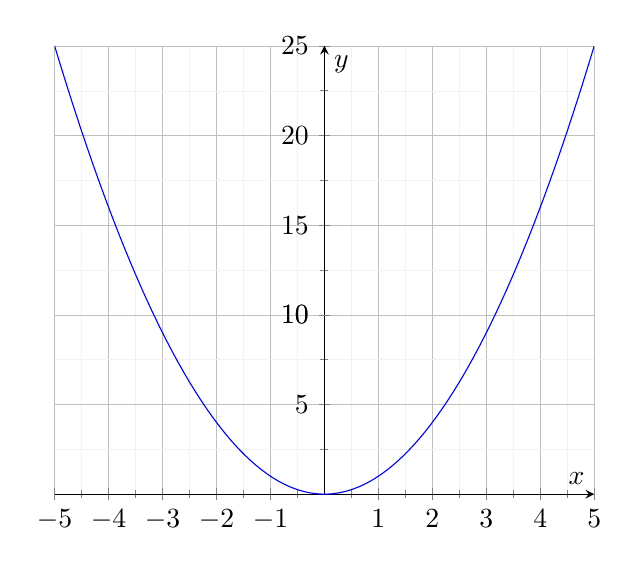
\begin{tikzpicture}
  \begin{axis}[
      xmin=-5, xmax=5,
      ymin=0, ymax=25,
      axis lines=middle,
      xlabel={$x$},
      ylabel={$y$},
      xtick={-5,-4,...,5}, % 表示从-5到5的整数
      ytick={0,5,...,25},
      extra y ticks={10}, % 额外的y轴刻度
      grid=both, % 显示网格
      grid style={line width=.1pt, draw=gray!10},
      major grid style={line width=.2pt,draw=gray!50},
      minor tick num=1 % 每个主刻度之间的次刻度数量
    ]
    \addplot[
      domain=-5:5, % 函数定义域
      samples=100, % 样本点数量
      color=blue, % 线条颜色
      ]
      {x^2}; % 函数表达式
  \end{axis}
\end{tikzpicture}
\caption{y=x*x}
\end{table}
\end{itemize}
\end{enumerate}
%1.1.7矩阵==================================================%
\subsubsection{矩阵}
\begin{enumerate}
  \item 矩阵
   \begin{itemize}
      \item 命令展示
\begin{lstlisting}
\[
 \mathbf{H}=
 \begin{bmatrix}
 \dfrac{\partial^2 f}{\partial x^2} &
 \dfrac{\partial^2 f}
 {\partial x \partial y} \\[8pt]
 \dfrac{\partial^2 f}
 {\partial x \partial y} &
 \dfrac{\partial^2 f}{\partial y^2}
 \end{bmatrix}
 \]
\end{lstlisting}
\item 效果展示
\[
 \mathbf{H}=
 \begin{bmatrix}
 \dfrac{\partial^2 f}{\partial x^2} &
 \dfrac{\partial^2 f}
 {\partial x \partial y} \\[8pt]
 \dfrac{\partial^2 f}
 {\partial x \partial y} &
 \dfrac{\partial^2 f}{\partial y^2}
 \end{bmatrix}
 \]
\end{itemize}
\end{enumerate}
%1.1.8页眉页脚==================================================%
\subsubsection{页眉页脚}
\begin{enumerate}
  \item 页眉页脚
   \begin{itemize}
      \item 命令展示
\begin{lstlisting}
\pagestyle{fancy}
\fancyhf{}
\renewcommand{\headrulewidth}{1pt}
\renewcommand{\footrulewidth}{1pt}
\fancyhead[L]{
\includegraphics[width=1.5cm]{okkl}} 
\fancyhead[C]{\rightmark}
\fancyfoot[C]{\thepage}
\fancyhead[R]{\thepage}


\end{lstlisting}
\item 效果展示
\begin{mdframed}
  \begin{minipage}{0.5\textwidth}
    
\includegraphics[width=\linewidth]{n1}
    \captionof{figure}{Image 1}
  \end{minipage}
  \hfill
  \begin{minipage}{0.5\textwidth}
    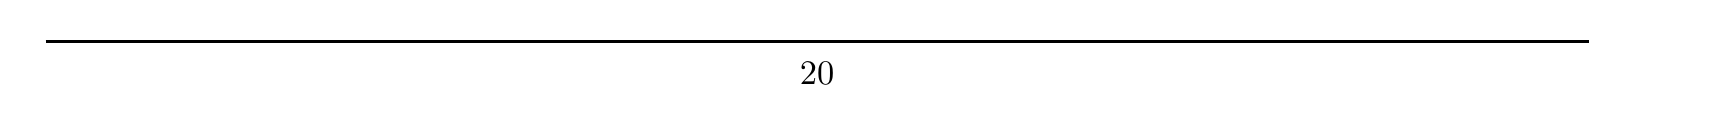
\includegraphics[width=\linewidth]{n2}
    \captionof{figure}{Image 2}
  \end{minipage}
\end{mdframed}

如文档所示
\end{itemize}
\end{enumerate}

%1.1.9并排图==================================================%
\subsubsection{并排图}
\begin{enumerate}
  \item 并排图
   \begin{itemize}
      \item 命令展示
\begin{lstlisting}
\begin{mdframed}
  \begin{minipage}{0.5\textwidth}
    
\includegraphics[width=\linewidth]{good}
    \captionof{figure}{Image 1}
  \end{minipage}
  \hfill
  \begin{minipage}{0.5\textwidth}
    
\includegraphics[width=\linewidth]{good}
    \captionof{figure}{Image 2}
  \end{minipage}
\end{mdframed}
\end{lstlisting}
\item 效果展示

\begin{mdframed}
  \begin{minipage}{0.5\textwidth}
    
\includegraphics[width=\linewidth]{good}
    \captionof{figure}{Image 1}
  \end{minipage}
  \hfill
  \begin{minipage}{0.5\textwidth}
    
\includegraphics[width=\linewidth]{good}
    \captionof{figure}{Image 2}
  \end{minipage}
\end{mdframed}
\end{itemize}
\end{enumerate}
%1.1.10三线表==================================================%
\subsubsection{三线表}
\begin{enumerate}
  \item 三线表
   \begin{itemize}
      \item 命令展示
\begin{lstlisting}
\begin{tabular}{cccc}
 \toprule
 & \multicolumn{3}{c}{Numbers} \\
 \cmidrule{2-4}
 & 1 & 2 & 3 \\
 \midrule
 Alphabet & A & B & C \\
 Roman
 Numbers
 1 2 3
 & I & II& III \\
 \bottomrule
 \end{tabular}
\end{lstlisting}
\item 效果展示
\begin{tabular}{cccc}
 \toprule
 & \multicolumn{3}{c}{Numbers} \\
 \cmidrule{2-4}
 & 1 & 2 & 3 \\
 \midrule
 Alphabet & A & B & C \\
 Roman
 Numbers
 1 2 3
 & I & II& III \\
 \bottomrule
 \end{tabular}
\end{itemize}
\end{enumerate}
%1.1.11嵌套表格==================================================%
\subsubsection{嵌套表格}
\begin{enumerate}
  \item 嵌套表格
   \begin{itemize}
      \item 命令展示
\begin{lstlisting}
\begin{tabular}{|c|c|c|}
 \hline
 a& b &c \\\hline
 a& \multicolumn{1}{@{}c@{}|}
 {\begin{tabular}{c|c}
 o &k \\ \hline
 o &k \\
 \end{tabular}}
 &c \\\hline
 a& b &c \\\hline
 \end{tabular}
\end{lstlisting}
\item 效果展示
\begin{tabular}{|c|c|c|}
 \hline
 a& b &c \\\hline
 a& \multicolumn{1}{@{}c@{}|}
 {\begin{tabular}{c|c}
 o &k \\ \hline
 o &k \\
 \end{tabular}}
 &c \\\hline
 a& b &c \\\hline
 \end{tabular}
\end{itemize}
\end{enumerate}
%1.1.12多行公式==================================================%
\subsubsection{多行公式}
\begin{enumerate}
  \item 多行公式
   \begin{itemize}
      \item 命令展示
\begin{lstlisting}
\begin{multline}
 a + b + c + d + e + f
 + g + h + i \\
 = j + k + l + m + n\\
 = o + p + q + r + s

 \end{multline}
\end{lstlisting}
\item 效果展示
\begin{multline}
 a + b + c + d + e + f
 + g + h + i \\
 = j + k + l + m + n\\
 = o + p + q + r + s
 \end{multline}
\end{itemize}
\end{enumerate}
%1.1.13按等号对齐的多行公式==================================================%
\subsubsection{按等号对齐的多行公式}
\begin{enumerate}
  \item 按等号对齐的多行公式
   \begin{itemize}
      \item 命令展示
\begin{lstlisting}
\begin{equation}
 \begin{aligned}
 a&= b+ c\\
 d&= e+ f+g\\
 h+i&= j+k\\
 l+m&= n
 \end{aligned}
 \end{equation}
\end{lstlisting}
\item 效果展示
\begin{equation}
 \begin{aligned}
 a&= b+ c\\
 d&= e+ f+g\\
 h+i&= j+k\\
 l+m&= n
 \end{aligned}
 \end{equation}
\end{itemize}
\end{enumerate}
%1.1.14分段函数==================================================%
\subsubsection{分段函数}
\begin{enumerate}
  \item 分段函数
   \begin{itemize}
      \item 命令展示
\begin{lstlisting}
\[ |x|= \left\{
 \begin{array}{rl}-x & x<0,\\
 0&x=0,\\
 x&x>0.
 \end{array}\right.\]
\end{itemize}
\end{lstlisting}
\item 效果展示
\[ |x|= \left\{
 \begin{array}{rl}-x & x<0,\\
 0&x=0,\\
 x&x>0.
 \end{array}\right.\]
\end{itemize}
\end{enumerate}
%1.1.15 证明环境和证毕符号==================================================%
\subsubsection{ 证明环境和证毕符号}
\begin{enumerate}
  \item  证明环境和证毕符号
   \begin{itemize}
      \item 命令展示
\begin{lstlisting}
\begin{proof}
 Assuming $\gamma
 = 1/\sqrt{1-v^2/c^2}$, then
 \begin{align*}
 E &= \gamma m_0 c^2 \\
 p &= \gamma m_0v \qedhere
 \end{align*}
 \end{proof}
\end{lstlisting}
\item 效果展示
\begin{proof}
 Assuming $\gamma
 = 1/\sqrt{1-v^2/c^2}$, then
 \begin{align*}
 E &= \gamma m_0 c^2 \\
 p &= \gamma m_0v \qedhere
 \end{align*}
 \end{proof}
\end{itemize}
\end{enumerate}
%1.1.16颜色的表达==================================================%
\subsubsection{颜色的表达}
\begin{enumerate}
  \item 例如
   \begin{itemize}
      \item 命令展示
\begin{lstlisting}
\large\sffamily
\color{red!40} 
\color{blue} 
\color{blue!50!black} 
\color{black} 
\end{lstlisting}
\item 效果展示
\large\sffamily
{\color{red!40} 40\% 红色}
{\color{blue} 蓝色}
{\color{blue!50!black} 蓝黑}
{\color{black} 黑色}
\end{itemize}
\end{enumerate}
%1.1.17超链接==================================================%
\subsubsection{超链接}
\begin{enumerate}
  \item 超链接
   \begin{itemize}
      \item 命令展示
\begin{lstlisting}
\href{https://github.com/KeepingMoving/work1.git}{GitHub}
\end{lstlisting}
\item 效果展示
\href{https://github.com/KeepingMoving/work1.git}{GitHub}
\end{itemize}
\end{enumerate}
%1.1.18积分图像==================================================%
\subsubsection{积分图像}
\begin{enumerate}
  \item 积分图像
   \begin{itemize}
      \item 命令展示
\begin{lstlisting}
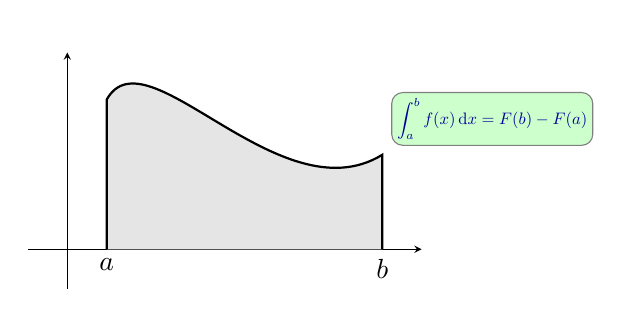
\begin{tikzpicture}
 \draw[-stealth,line width=0.2pt] (-0.5,0)-- (4.5,0);
 \draw[-stealth,line width=0.2pt] (0,-0.5)-- (0,2.5);
 \coordinate (a) at (0.5,1.9);
 \coordinate (b) at (4,1.2);
 \node[below] (a0) at (a |- 0,0) {$a$};
 \node[below] (b0) at (b |- 0,0) {$b$};
 \filldraw[fill=gray!20,draw,thick]
 (a0)-- (a) .. controls (1,2.8) and (2.7,0.4) .. (b)-- (b0)-- cycle;
 \node[above right,outer sep=0.2cm, rounded corners,
 fill=green!20,draw=gray,text=blue!60!black,scale=0.6]
 at (b) {$\displaystyle \int_a^b {f(x)\,\mathrm{d}x} = F(b)- F(a)$};
 \end{tikzpicture}
\end{lstlisting}
\item 效果展示
\begin{table}[H]
\centering
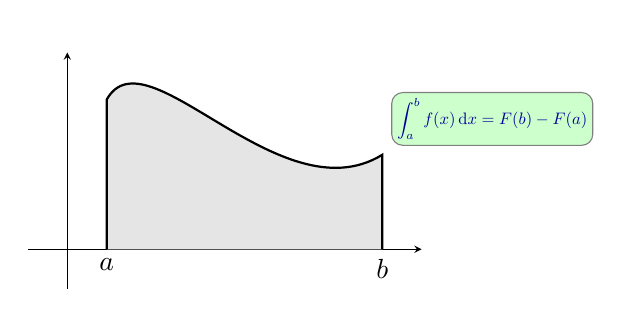
\begin{tikzpicture}
 \draw[-stealth,line width=0.2pt] (-0.5,0)-- (4.5,0);
 \draw[-stealth,line width=0.2pt] (0,-0.5)-- (0,2.5);
 \coordinate (a) at (0.5,1.9);
 \coordinate (b) at (4,1.2);
 \node[below] (a0) at (a |- 0,0) {$a$};
 \node[below] (b0) at (b |- 0,0) {$b$};
 \filldraw[fill=gray!20,draw,thick]
 (a0)-- (a) .. controls (1,2.8) and (2.7,0.4) .. (b)-- (b0)-- cycle;
 \node[above right,outer sep=0.2cm, rounded corners,
 fill=green!20,draw=gray,text=blue!60!black,scale=0.6]
 at (b) {$\displaystyle \int_a^b {f(x)\,\mathrm{d}x} = F(b)- F(a)$};
 \end{tikzpicture}
\end{table}
\end{itemize}
\end{enumerate}
%1.1.19文字结点==================================================%
\subsubsection{文字结点}
\begin{enumerate}
  \item 文字结点
   \begin{itemize}
      \item 命令展示
\begin{lstlisting}
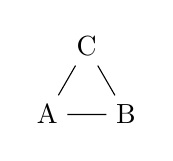
\begin{tikzpicture}
 \node (A) at (0,0) {A};
 \node (B) at (1,0) {B};
 \node (C) at (60:1) {C};
 \draw (A)-- (B)-- (C)-- (A);
 \end{tikzpicture}
\end{lstlisting}
\item 效果展示
\begin{table}
\centering
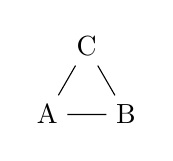
\begin{tikzpicture}
 \node (A) at (0,0) {A};
 \node (B) at (1,0) {B};
 \node (C) at (60:1) {C};
 \draw (A)-- (B)-- (C)-- (A);
 \end{tikzpicture}
\end{table}
\end{itemize}

\end{enumerate}

%1.1.20循环==================================================%


\subsubsection{循环}
\begin{enumerate}
  \item 有序列表(enumerate)
   \begin{itemize}
      \item 命令展示
\begin{lstlisting}
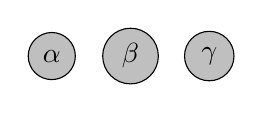
\begin{tikzpicture}
 \foreach \n/\t in
 {0/\alpha,1/\beta,2/\gamma}
 {\node[circle,fill=lightgray,draw]
 at (\n,0) {$\t$};}
 \end{tikzpicture}
 \end{tikzpicture}
\end{lstlisting}
\item 效果展示
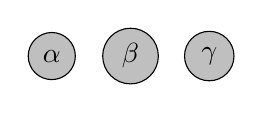
\begin{tikzpicture}
 \foreach \n/\t in
 {0/\alpha,1/\beta,2/\gamma}
 {\node[circle,fill=lightgray,draw]
 at (\n,0) {$\t$};}
 \end{tikzpicture}
\end{itemize}
\end{enumerate}











%1.2git=========================================================================%
  \subsection{git}
  {\color{blue}git命令展示}




%1.2.1新建 Git 仓库并克隆==================================================%
\subsubsection{新建 Git 仓库并克隆}

  \begin{itemize} 
  
      \item 命令展示

git init 新建 Git 仓库\\
git clone https://github.com/KeepingMoving/work1.git 克隆
   \item 效果展示

\begin{figure}[H]
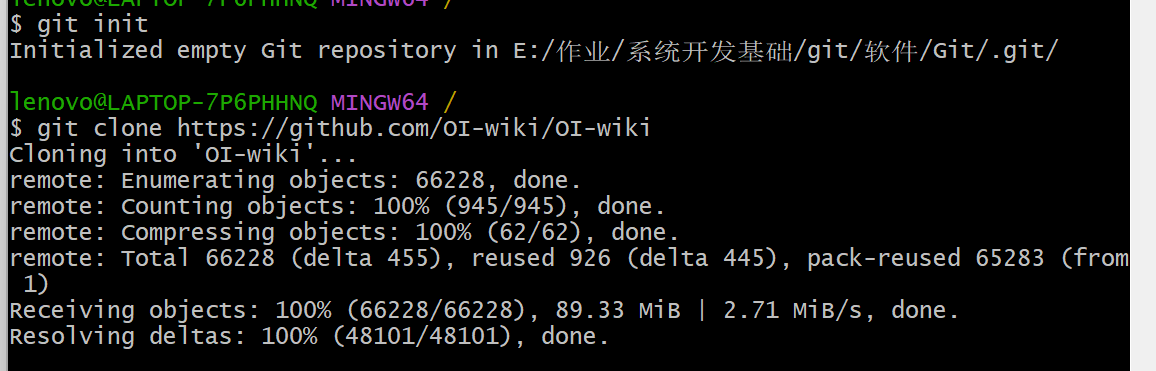
\includegraphics[width=1\textwidth]{a}
\end{figure}

\end{itemize}


%1.2.2跟踪文件==================================================%
\subsubsection{跟踪文件}

\begin{itemize}
  \item 命令展示
 
     git status 查看当前仓库文件的状态。\\
     git add     将指定的文件纳入到版本跟踪中
\item 效果展示
\begin{figure}[H]
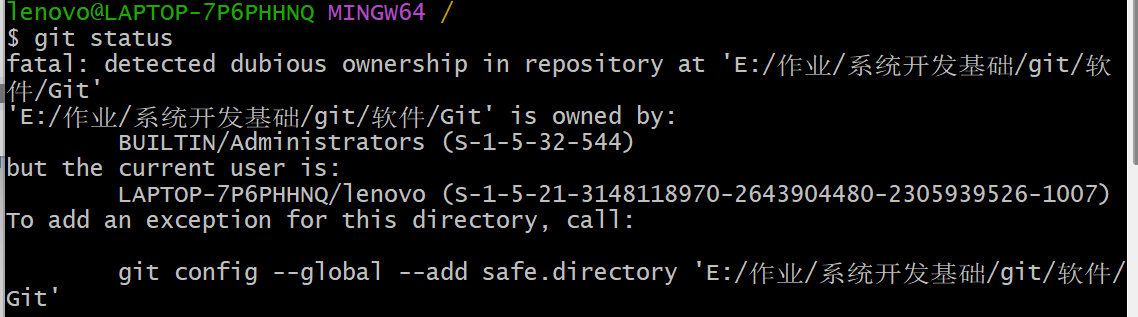
\includegraphics[width=1\textwidth]{2}
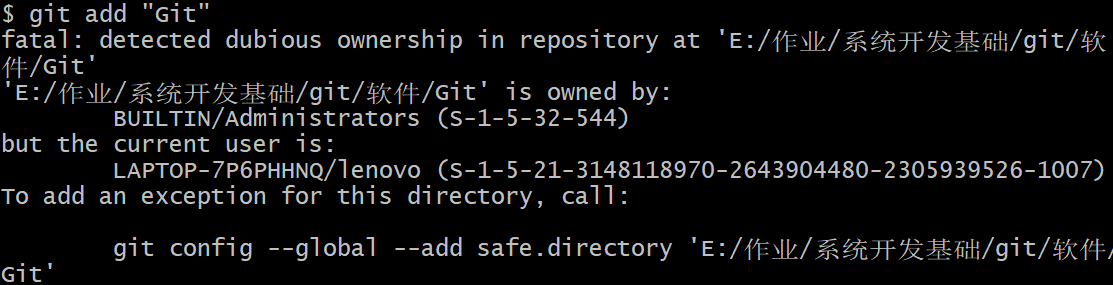
\includegraphics[width=1\textwidth]{3}
\end{figure}
\end{itemize}

%1.2.3修复最近的提交,但不创建新提交==================================================%
\subsubsection{分支}
\begin{itemize}
  \item 命令展示
 
     git branch 命令可以创建分支\\
     git switch 命令可以切换分支\\
     git switch -c 命令可以创建分支并切换到这个新分支。
\item 效果展示
 \begin{figure}[H]
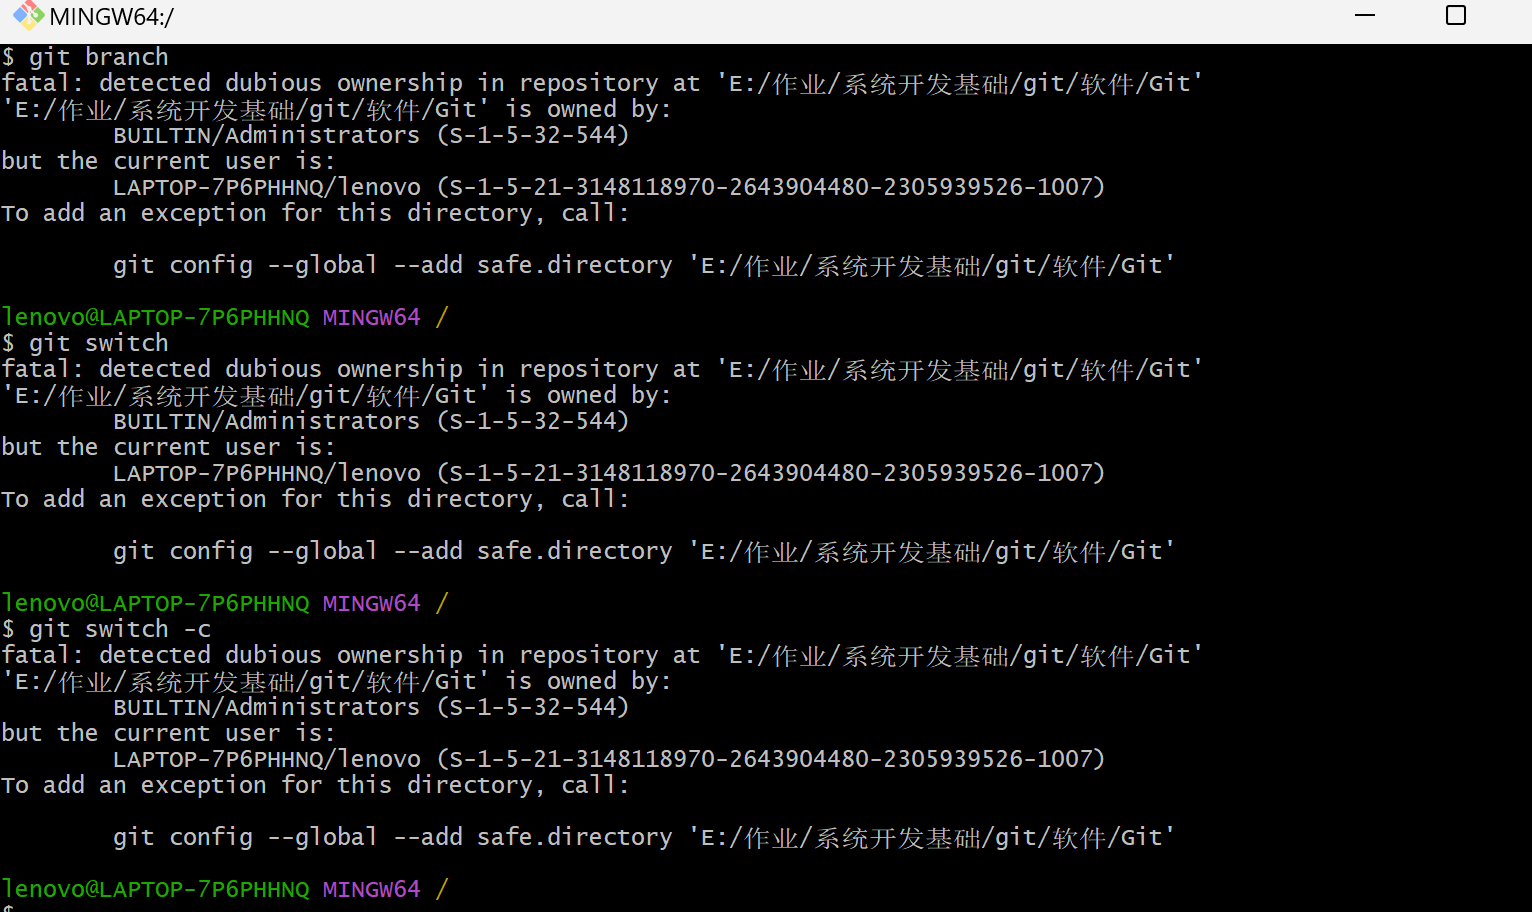
\includegraphics[width=1\textwidth]{4}
\end{figure}
\end{itemize}

%1.2.4表格==================================================%
\subsubsection{分支的合并}
\begin{itemize}
  \item 命令展示
 
     git merge 命令可以将该分支合并到当前分支上
\item 效果展示
 \begin{figure}[H]
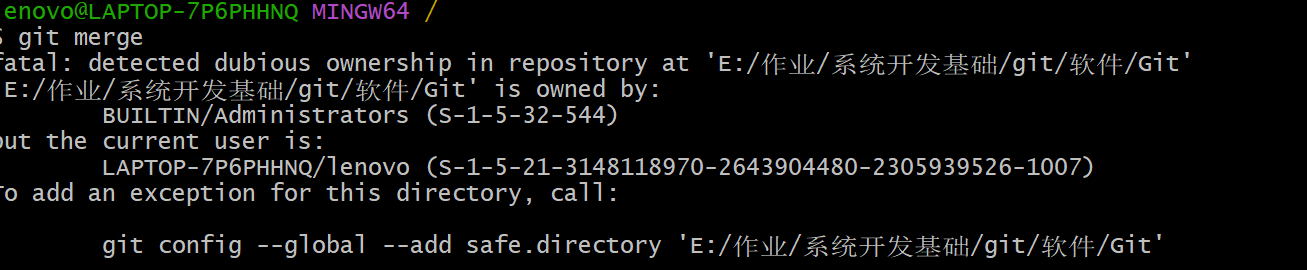
\includegraphics[width=1\textwidth]{5}
\end{figure}
\end{itemize}
%1.2.5表格==================================================%
\subsubsection{修复最近的提交,但不创建新提交}
\begin{itemize}
  \item 命令展示
 git reset --soft HEAD~1\\
git commit --amend
\item 效果展示
  \begin{figure}[H]
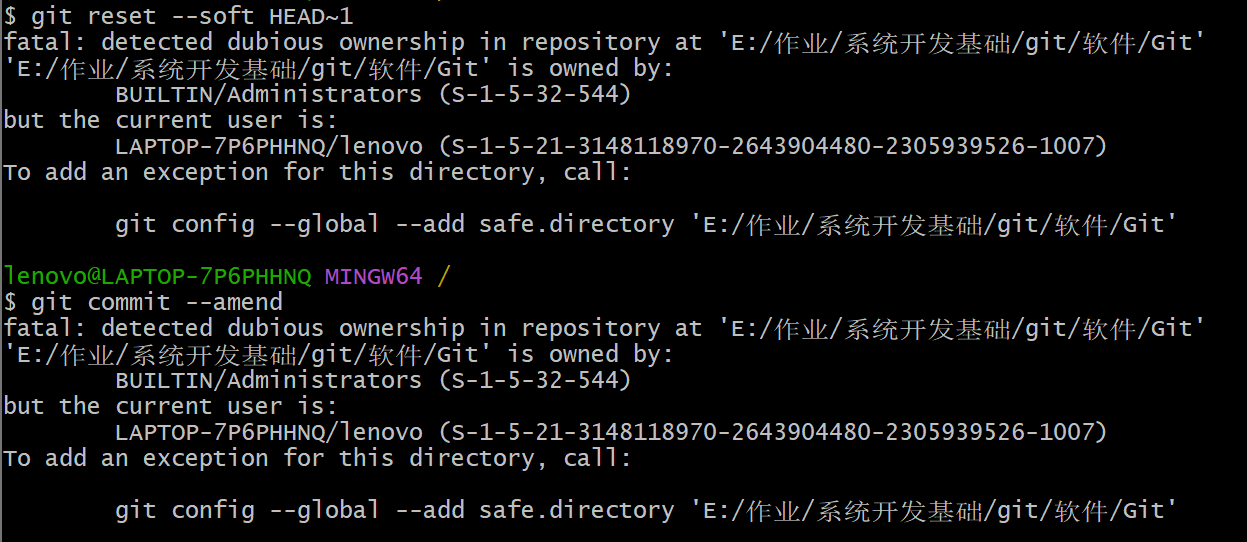
\includegraphics[width=1\textwidth]{6}
\end{figure}
\end{itemize}
%1.2.6表格==================================================%
\subsubsection{变基一个分支到另一个分支,并解决可能出现的冲突:}
\begin{itemize}
  \item 命令展示
 
     git checkout feature \\
     git rebase master\\
      如果有冲突,解决它们\\
    git add <resolved-files>\\
    git rebase --continue
\item 效果展示
   \begin{figure}[H]
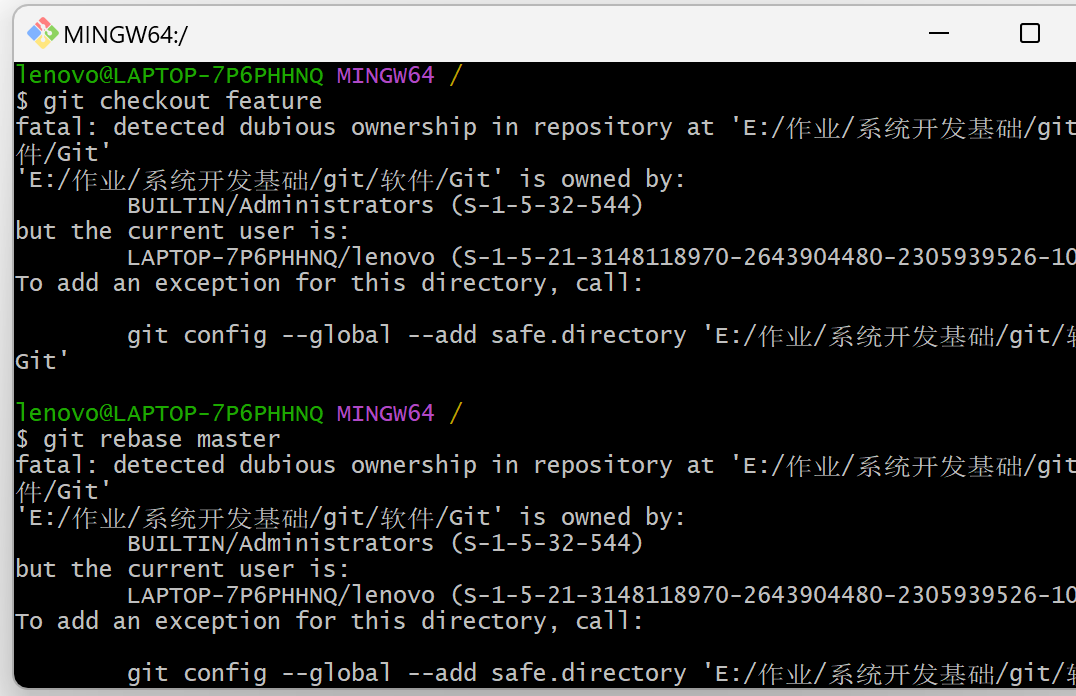
\includegraphics[width=1\textwidth]{30}
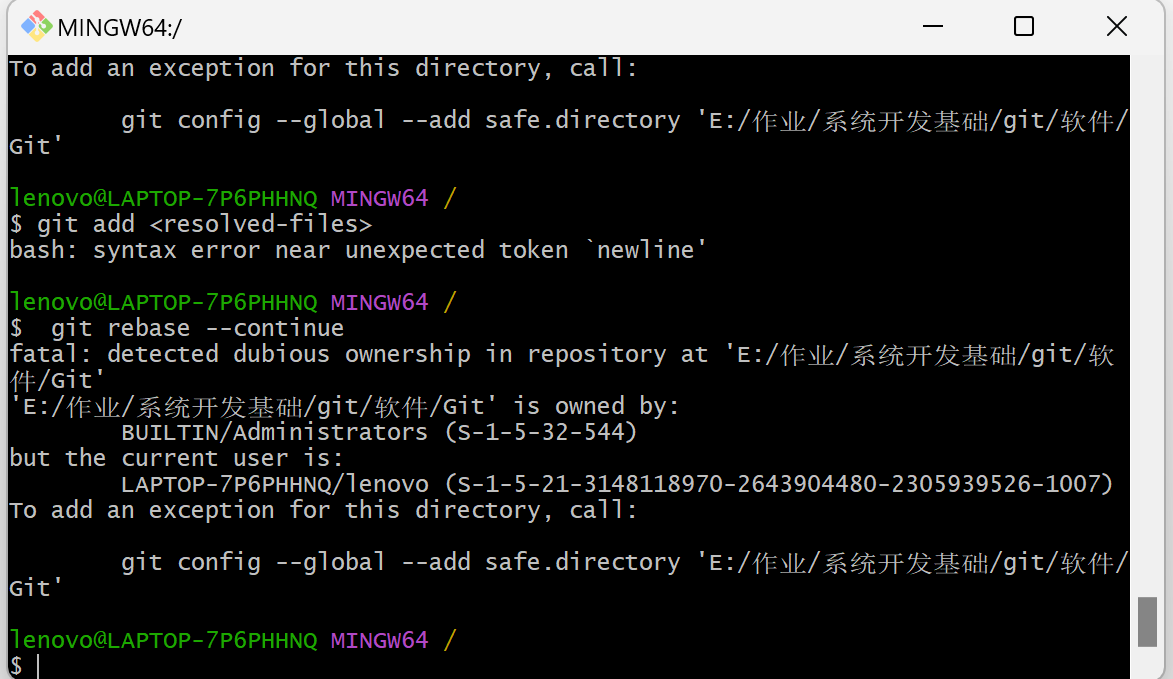
\includegraphics[width=1\textwidth]{31}
\end{figure}
\end{itemize}
%1.2.7表格==================================================%
\subsubsection{重写分支历史,使所有提交都成为主分支的一部分::}
\begin{itemize}
  \item 命令展示
 
git checkout experiment       切换到实验分支\\
git rebase -i master          交互式变基到主分支\\
  编辑交互式变基的提交列表,保存退出\\
git checkout master           切换回主分支\\
git merge experiment          合并实验分支
\item 效果展示
   \begin{figure}[H]
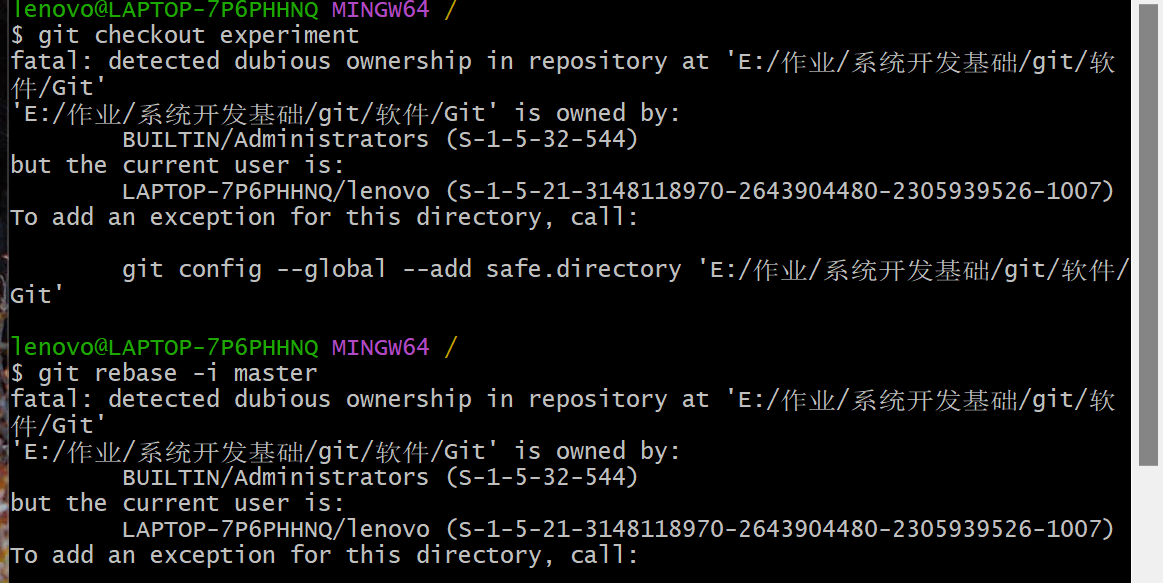
\includegraphics[width=1\textwidth]{9}
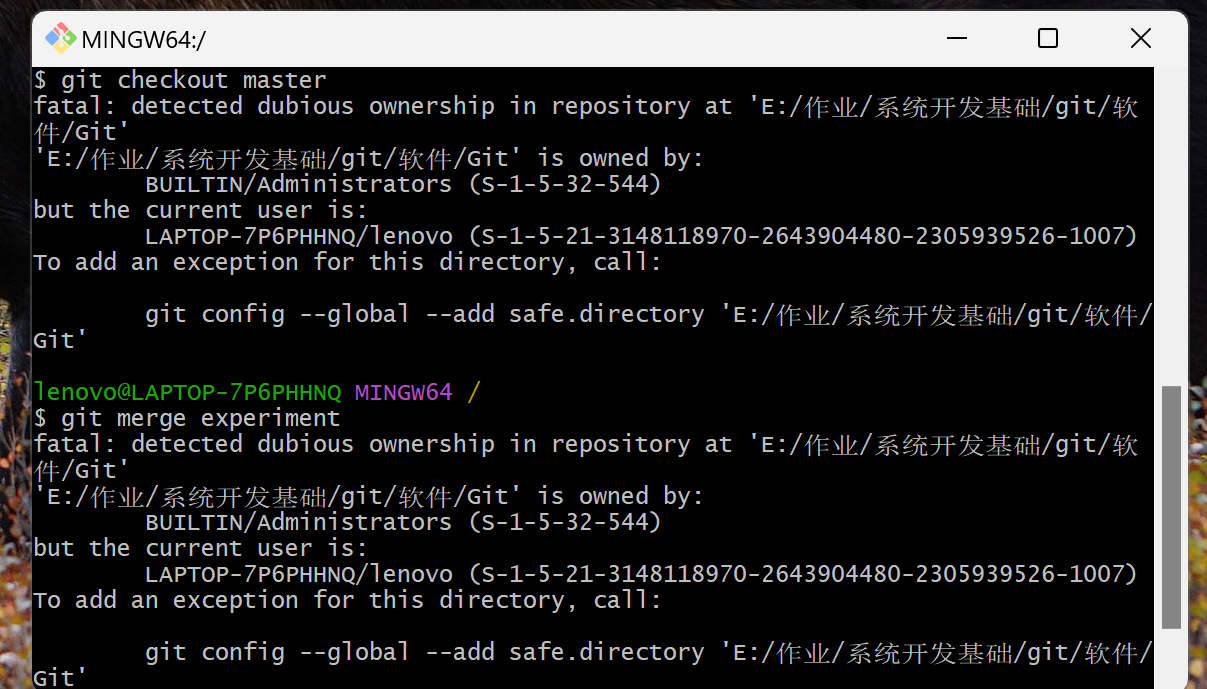
\includegraphics[width=1\textwidth]{10}
\end{figure}
\end{itemize}
%1.2.8表格==================================================%
\subsubsection{使用 grep 搜索提交历史中的特定文本}
\begin{itemize}
  \item 命令展示
 
    git log --pretty=format:"%h %s" | grep "search-text"    搜索提交信息中包含特定文本的提交

\item 效果展示
  \begin{figure}[H]
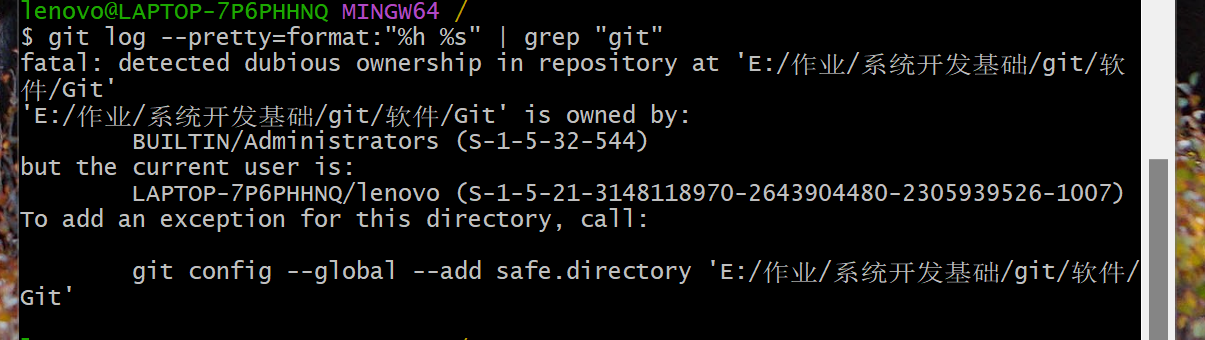
\includegraphics[width=1\textwidth]{11}
\end{figure}
\end{itemize}
%1.2.9表格==================================================%
\subsubsection{交互式变基并修改一系列提交}
\begin{itemize}
  \item 命令展示
 git checkout feature-branch  切换到功能分支\\
git rebase -i HEAD~5          交互式变基最近5个提交\\
  编辑交互式变基的提交列表,选择要修改的提交\\
git add "file"             添加修改后的文件\\
git rebase --continue       继续变基\\
\item 效果展示
  \begin{figure}[H]
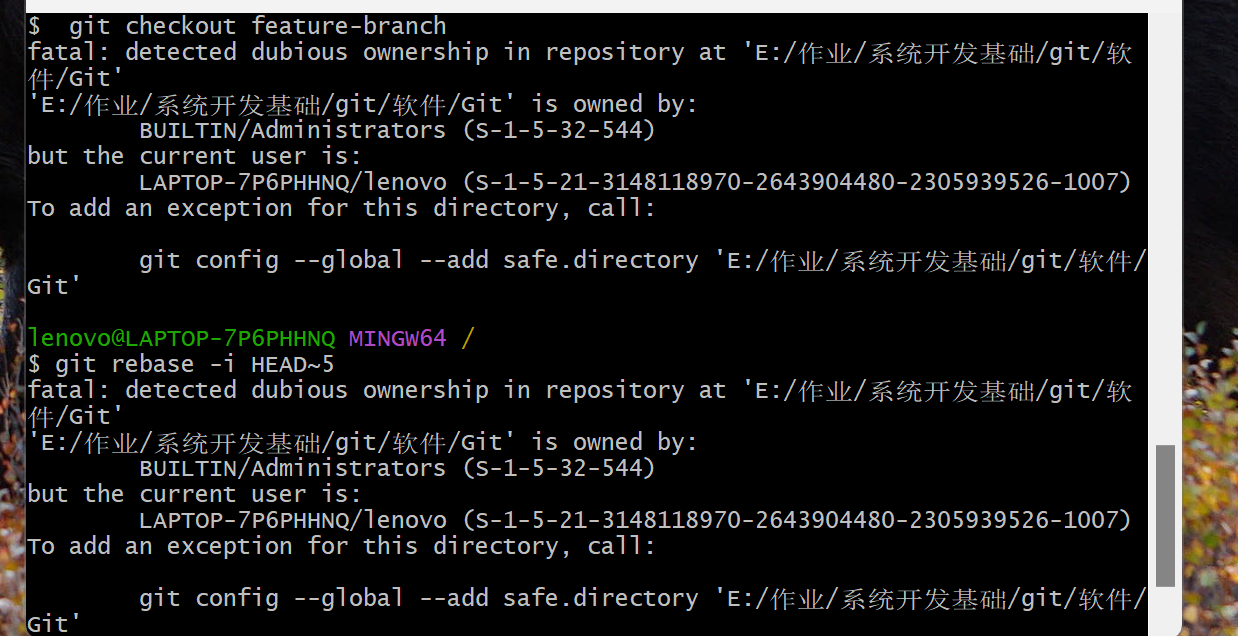
\includegraphics[width=1\textwidth]{12}
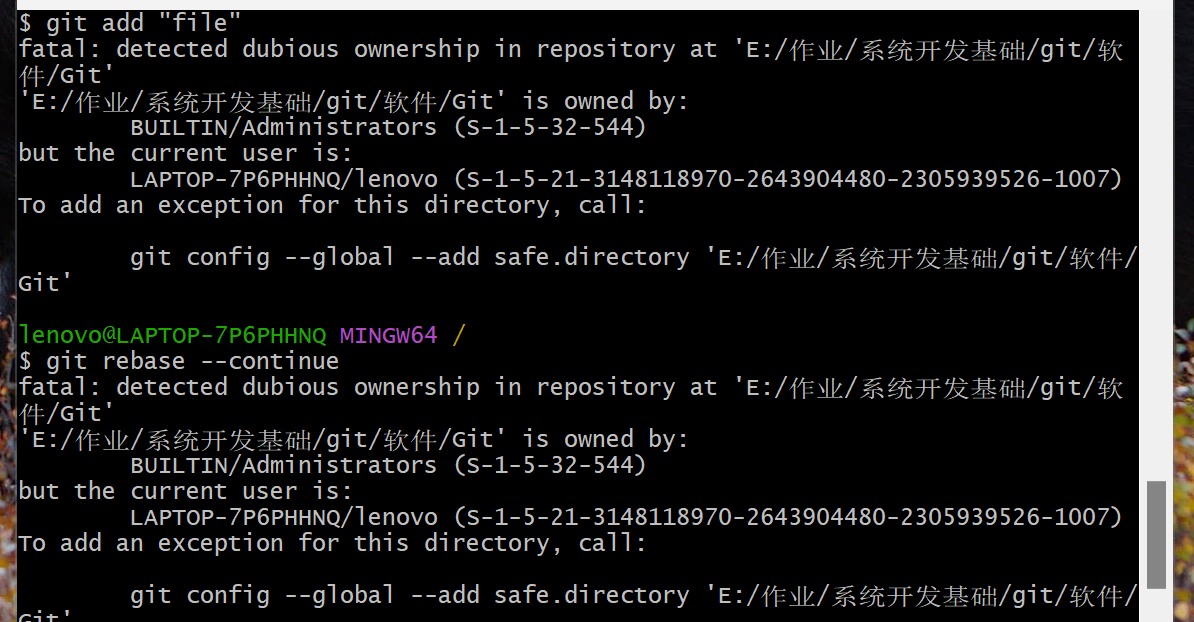
\includegraphics[width=1\textwidth]{13}
\end{figure}
\end{itemize}
%1.2.10表格==================================================%
\subsubsection{交互式变基并修改一系列提交}
\begin{itemize}
  \item 命令展示
  \begin{verbatim}
    #!/bin/bash
    commit_to_pick=$1  # 第一个参数是提交哈希
    git checkout master  # 切换到主分支
    if git cherry-pick $commit_to_pick; then
      echo "Cherry-pick successful."
    else
      echo "Cherry-pick failed, aborting."
      git cherry-pick --abort
    fi
  \end{verbatim}

  \item 效果展示
  \begin{figure}[H]
    \centering
    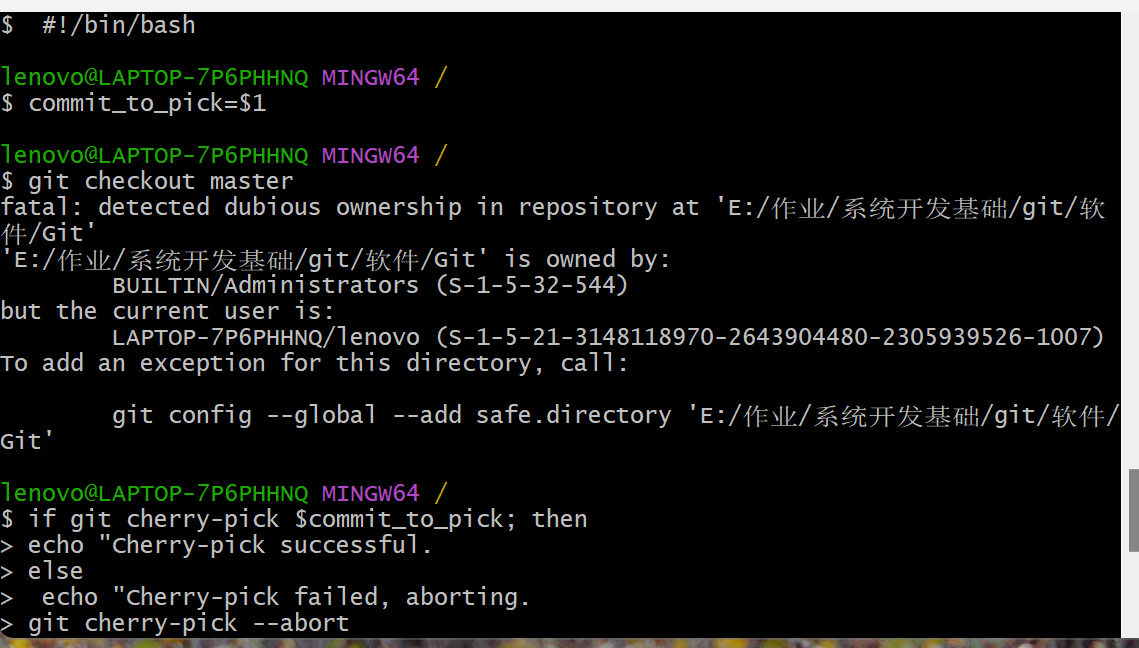
\includegraphics[width=\textwidth]{14} % 确保文件名正确
    \caption{交互式变基的效果展示}
    \label{fig:interactive-rebase}
  \end{figure}
\end{itemize}
%1.2.11表格==================================================%
\subsubsection{使用脚本自动化 Pull Request 合并流程}\begin{itemize}
  \item 命令展示
  \begin{verbatim}
    $ /bin/bash
    $ pr_branch=1                  # 第一个参数是 PR 分支名
    $ git fetch origin                # 获取远程分支
    $ git checkout pr_branch        # 切换到 PR 分支
    if git merge origin/master; then
      $ git push origin pr_branch
    else
      echo "Merge conflict detected."
    fi
  \end{verbatim}
\item 效果展示
\begin{figure}[H]
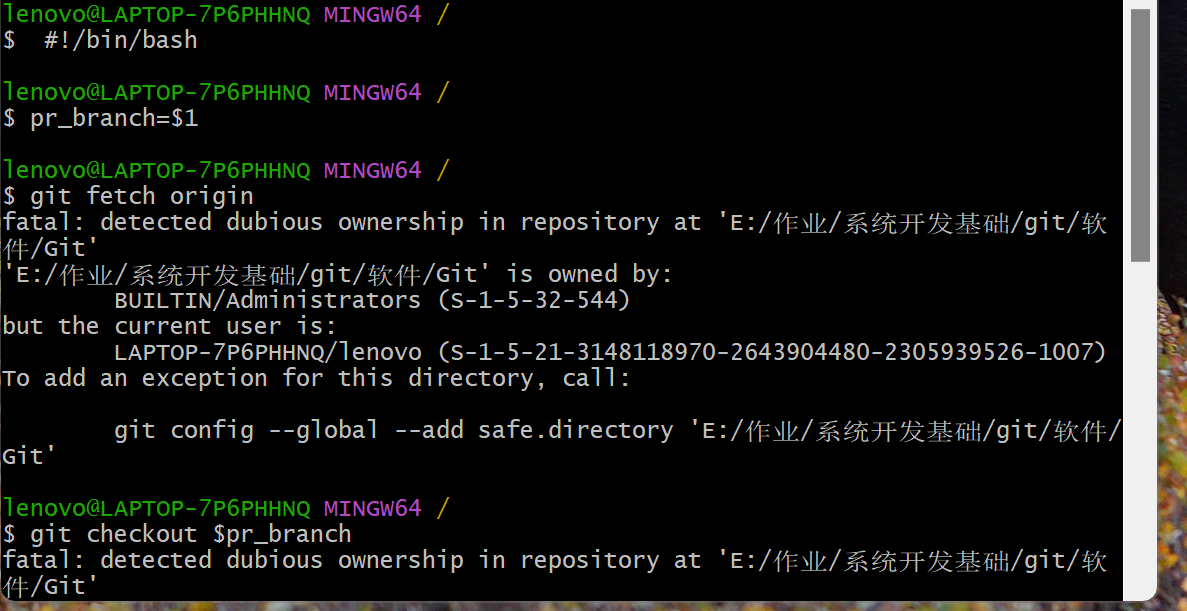
\includegraphics[width=1\textwidth]{16}
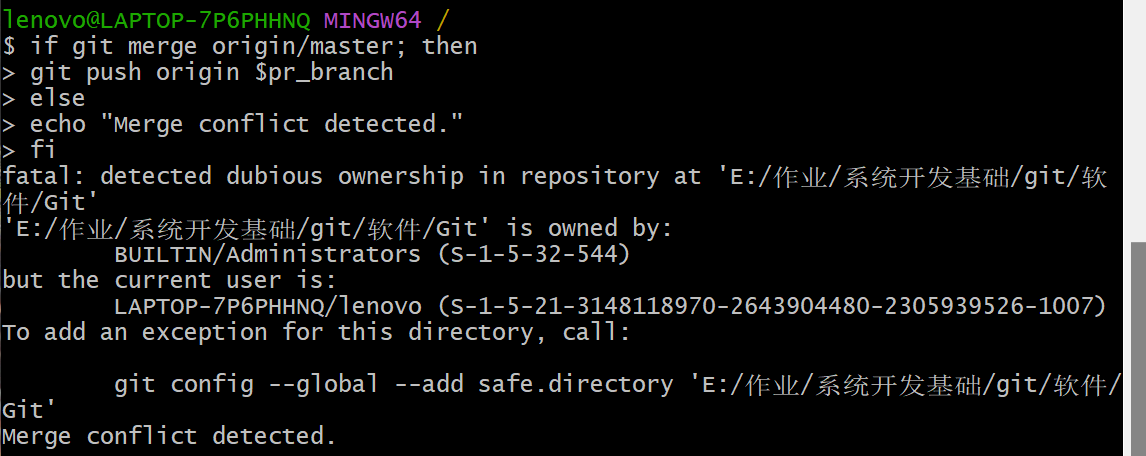
\includegraphics[width=1\textwidth]{17}
\end{figure}
\end{itemize}
%1.2.12表格==================================================%
\subsubsection{创建一个标签的自动化脚本}
\begin{itemize}
  \item 命令展示
  \begin{verbatim}
    #!/bin/bash
    tag_name=$1  # 第一个参数是标签名
    git checkout master  # 切换到主分支
    git pull           # 拉取最新代码
    git tag -a $tag_name -m "Tagging release"  # 创建带注释的标签
    git push origin $tag_name  # 推送标签到远程仓库
  \end{verbatim}

  \item 效果展示
  \begin{figure}[H]
    \centering
    % 展示三个并排的图像
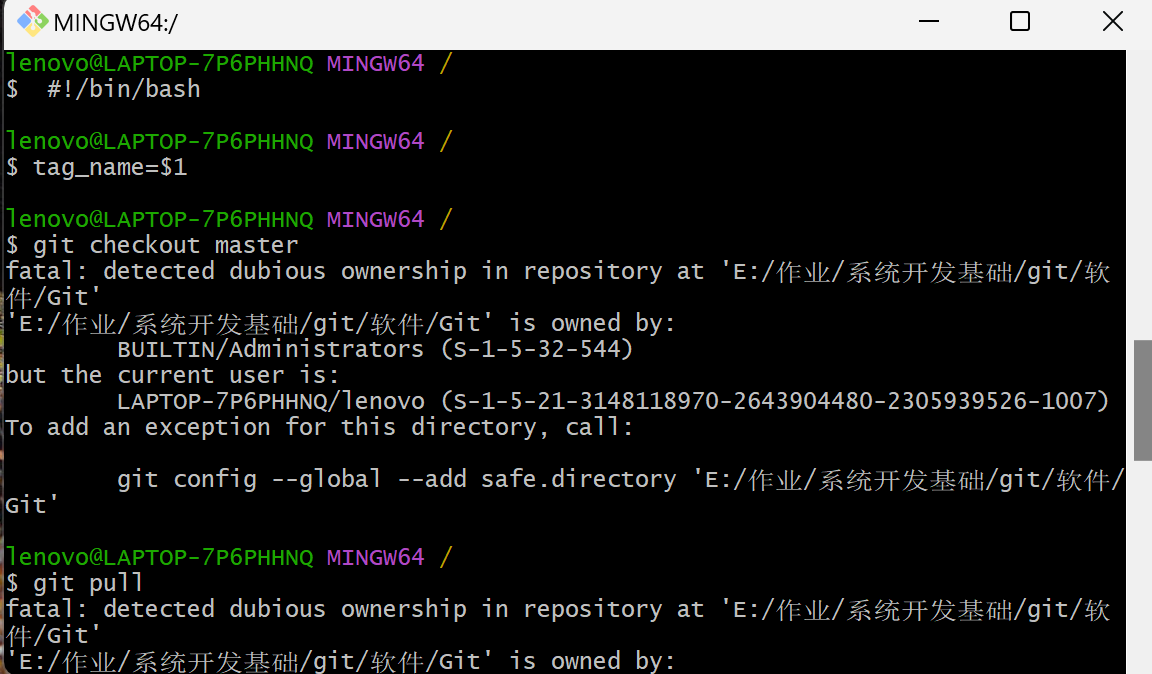
\includegraphics[width=1\textwidth]{18}
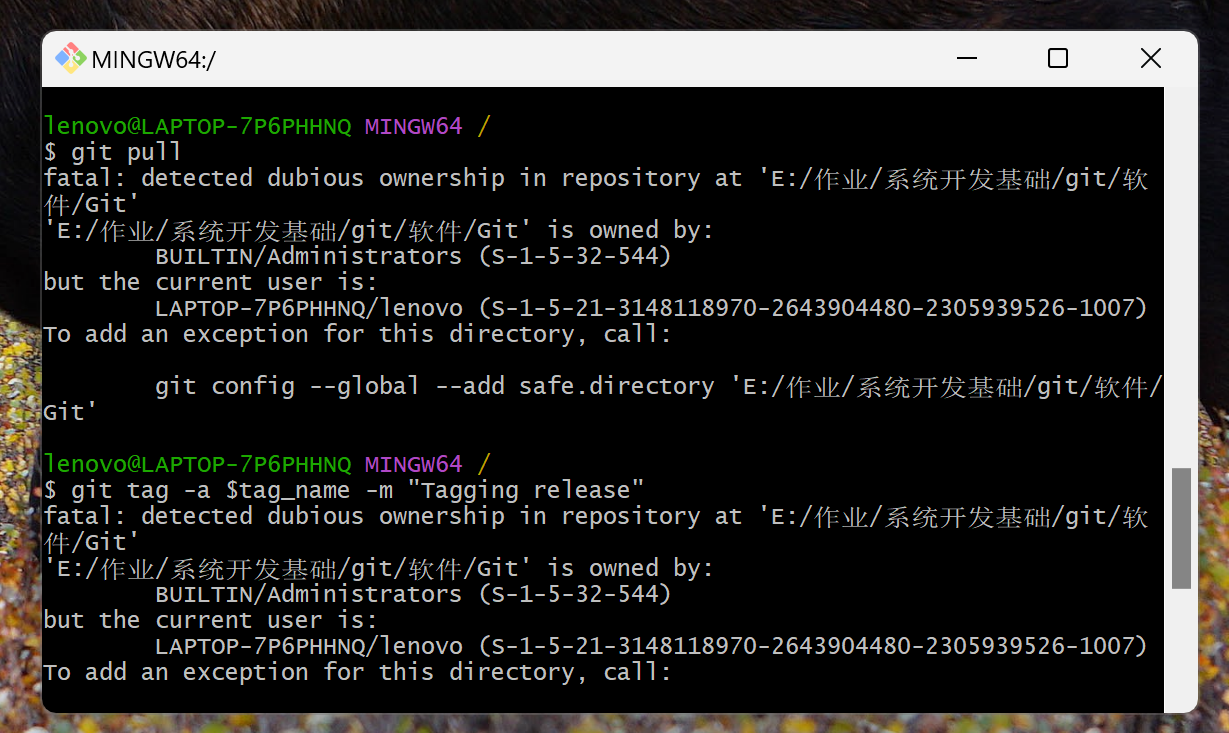
\includegraphics[width=1\textwidth]{19}
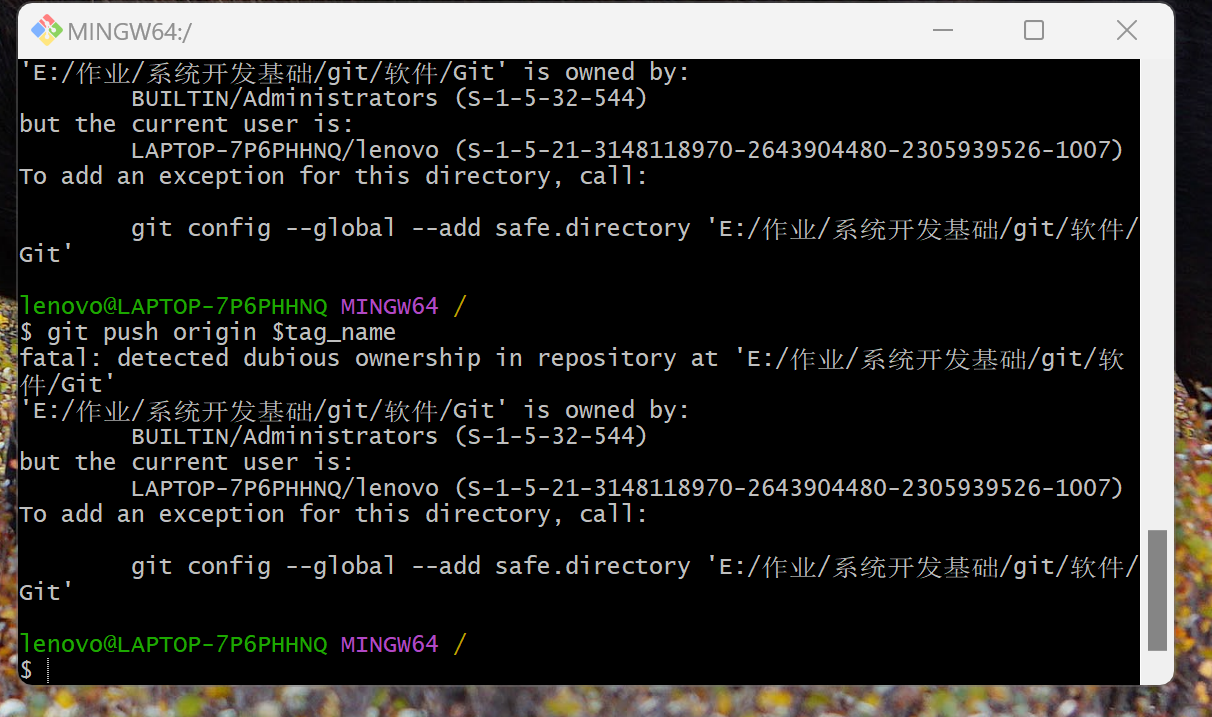
\includegraphics[width=1\textwidth]{20}

  \end{figure}
\end{itemize}

%1.2.13表格==================================================%
\subsubsection{使用脚本自动化删除过时的分支}
\begin{itemize}
  \item 命令展示
  \begin{verbatim}
    #!/bin/bash
    git fetch --all  # 获取所有分支信息
    for branch in `git for-each-ref --format='%(refname:short)' refs/remotes/origin/`; do
      if [[ $(git for-each-ref --format='%(upstream:short)' refs/heads/$branch) != "origin/$branch" ]]; then
        git branch --delete $branch
      fi
    done
  \end{verbatim}

  \item 效果展示
  \begin{figure}[H]
    \centering
    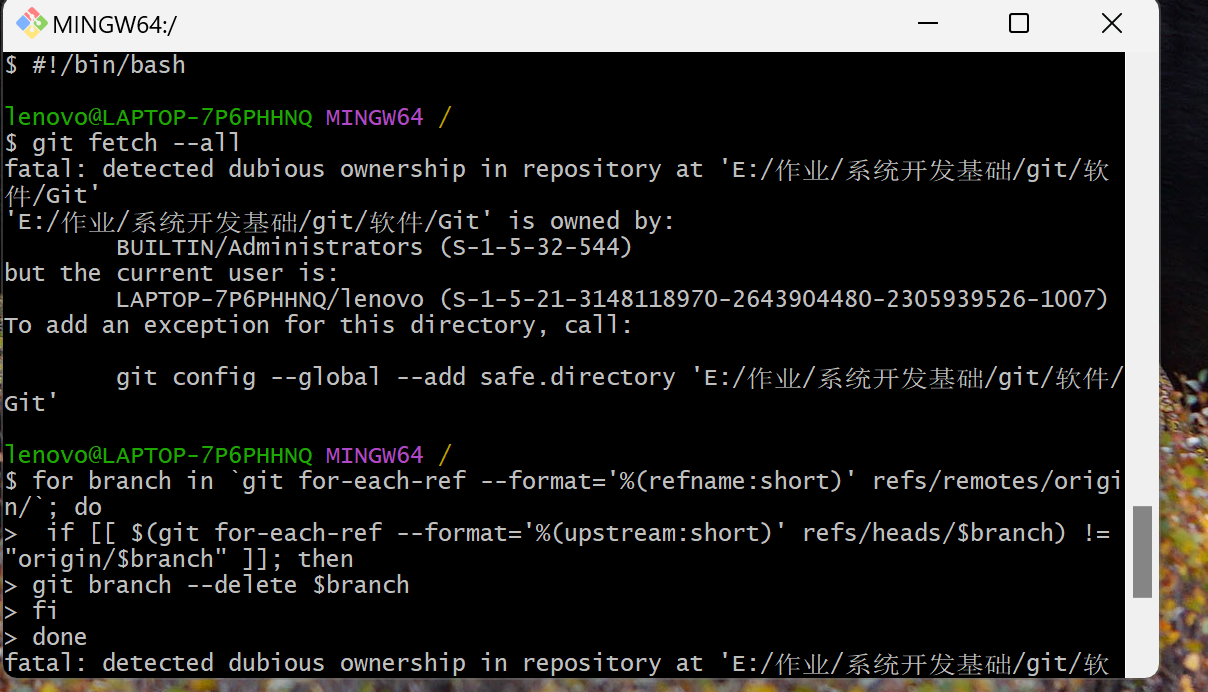
\includegraphics[width=\textwidth]{21} % 确保文件名正确
    \caption{自动化删除过时分支的效果展示}
    \label{fig:delete-branches}
  \end{figure}
\end{itemize}
%1.2.14表格==================================================%
\subsubsection{使用脚本自动化检查分支是否落后于远程分支}
\begin{itemize}
  \item 命令展示
  \begin{verbatim}
    #!/bin/bash
    git fetch origin  # 抓取远程分支
    for branch in `git for-each-ref --format='%(refname:short)' refs/heads/`; do
      if git rev-list --count --left-right origin/master...$branch; then
        echo "$branch is behind origin/master"
      fi
    done
  \end{verbatim}

  \item 效果展示
  \begin{figure}[H]
    \centering
    % 展示两个并排的图像
    \begin{minipage}{0.5\textwidth}
      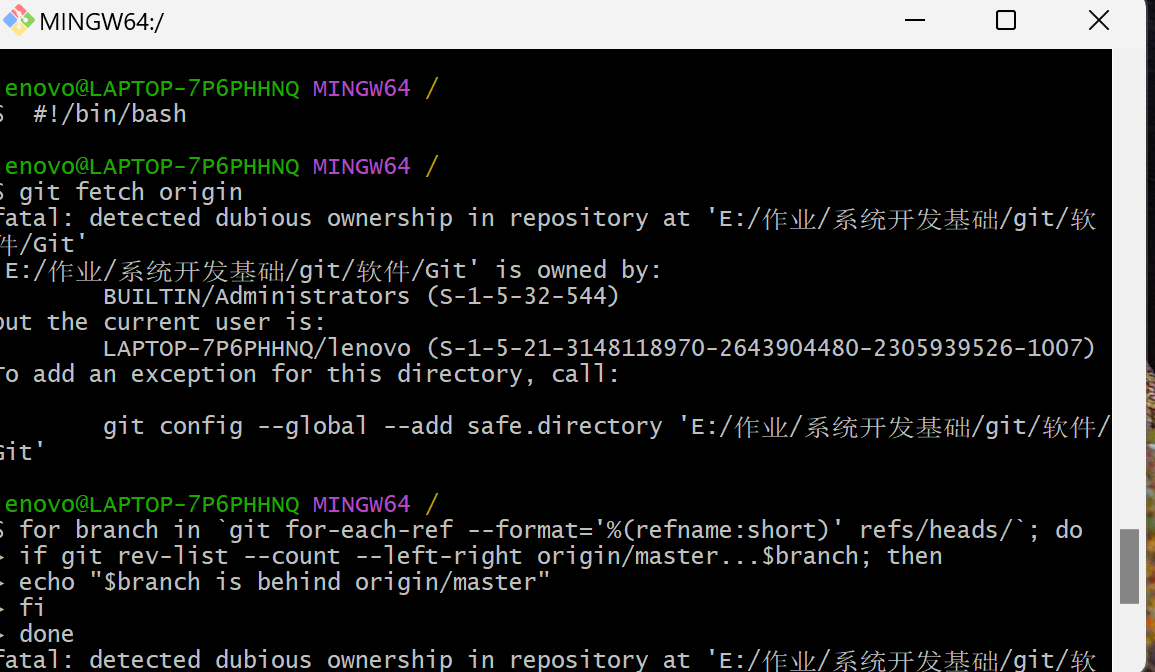
\includegraphics[width=\linewidth]{22}
      \caption{效果展示1}
      \label{fig:branch-comparison-1}
    \end{minipage}%
    \begin{minipage}{0.5\textwidth}
      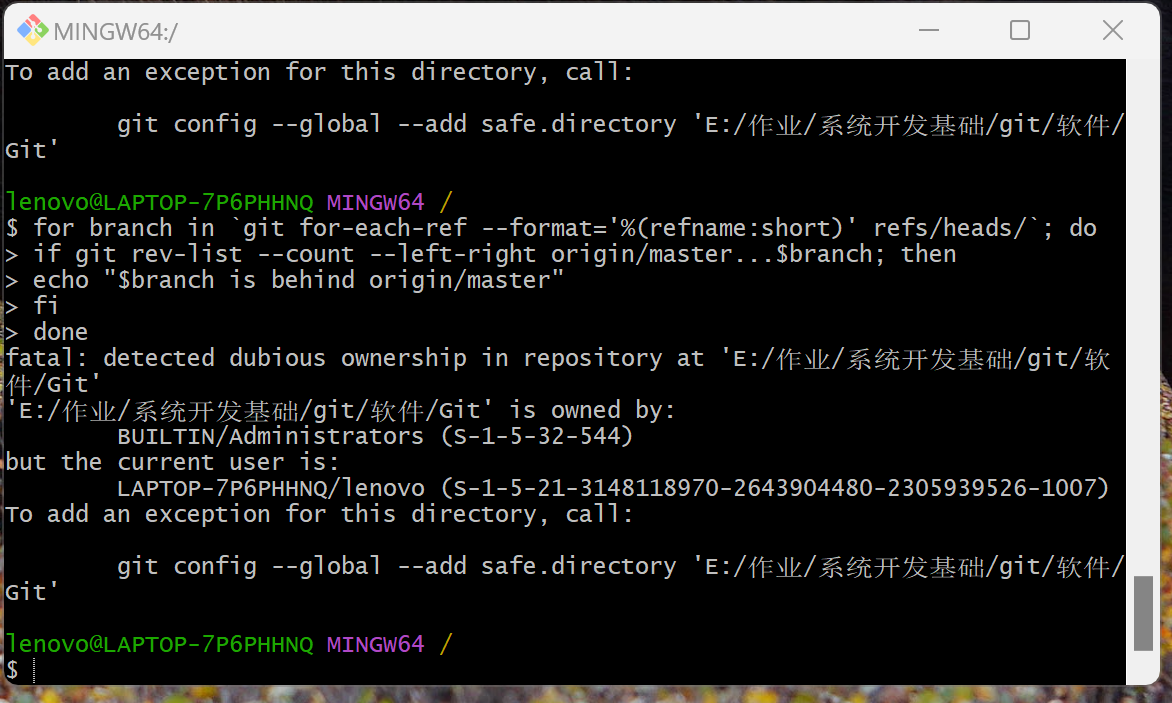
\includegraphics[width=\linewidth]{23}
      \caption{效果展示2}
      \label{fig:branch-comparison-2}
    \end{minipage}
    \caption{自动化检查分支是否落后于远程分支的效果展示}
    \label{fig:branch-check}
  \end{figure}
\end{itemize}
%1.2.15表格==================================================%
\subsubsection{检查Git仓库中是否有未提交的更改}
\begin{itemize}
  \item 命令展示
  \begin{verbatim}
    #!/bin/bash
    if git diff-index --name-only HEAD | read; then
      echo "You have uncommitted changes."
      git status
    else
      echo "No uncommitted changes."
    fi
  \end{verbatim}

  \item 效果展示
  \begin{figure}[H]
    \centering
    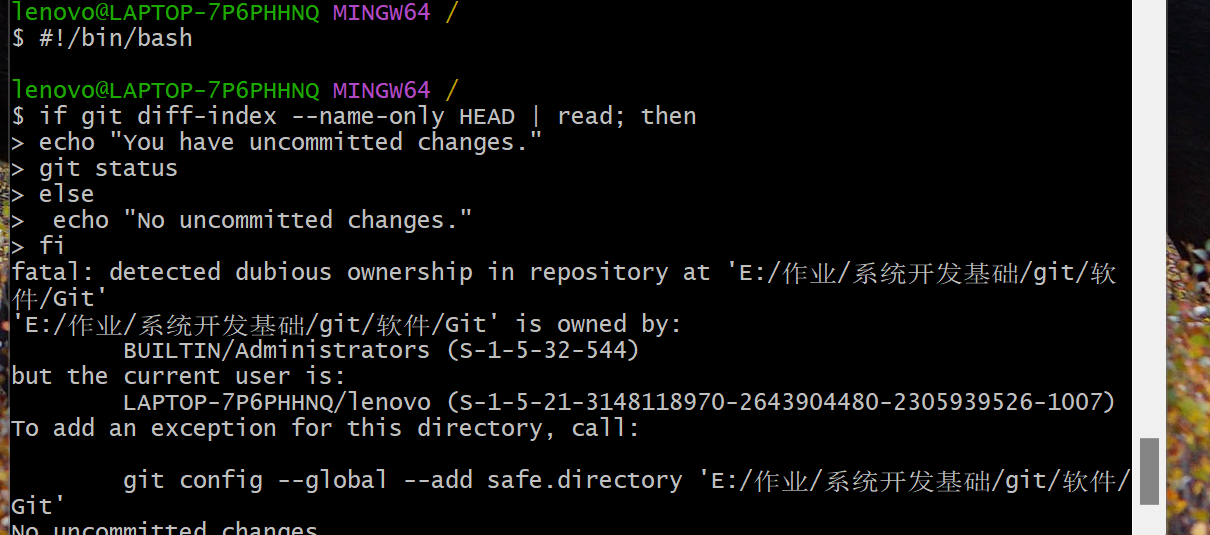
\includegraphics[width=\textwidth]{24} % 确保文件名正确
    \caption{检查未提交文件的效果展示}
    \label{fig:uncommitted-changes}
  \end{figure}
\end{itemize}
%1.2.16表格==================================================%
\subsubsection{使用脚本自动化检查远程分支是否存在}
\begin{itemize}
  \item 命令展示
  \begin{verbatim}
    #!/bin/bash
    remote_branch=$1  # 第一个参数是远程分支名
    if git show-ref --verify --quiet "refs/remotes/origin/$remote_branch"; then
      echo "Remote branch $remote_branch exists."
    else
      echo "Remote branch $remote_branch does not exist."
    fi
  \end{verbatim}

  \item 效果展示
  \begin{figure}[H]
    \centering
    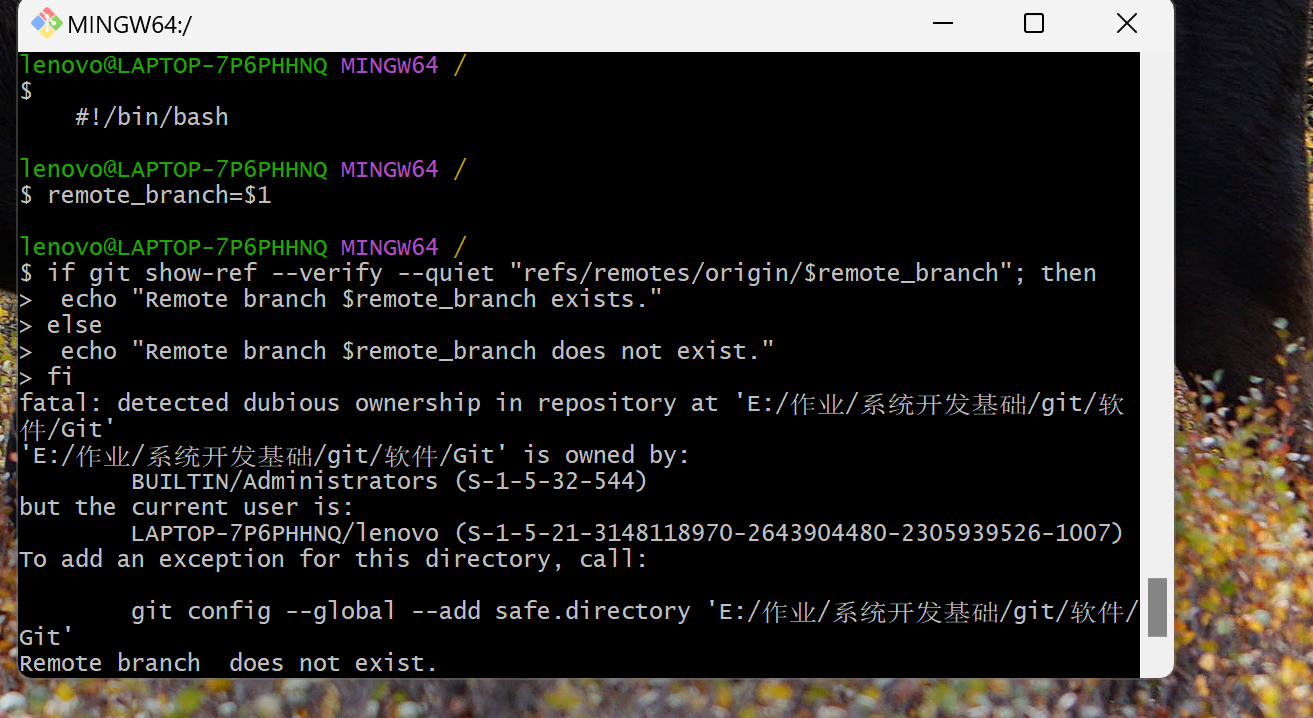
\includegraphics[width=\textwidth]{25} % 确保文件名正确
    \caption{检查远程分支是否存在的效果展示}
    \label{fig:remote-branch-check}
  \end{figure}
\end{itemize}


%1.2.16表格==================================================%

\subsubsection{使用命令来添加别名}
\begin{itemize}
  \item 命令展示
  \begin{verbatim}
    git config --global alias.graph "log --all --graph --decorate --oneline"

  \end{verbatim}

  \item 效果展示
  \begin{figure}[H]
    \centering
    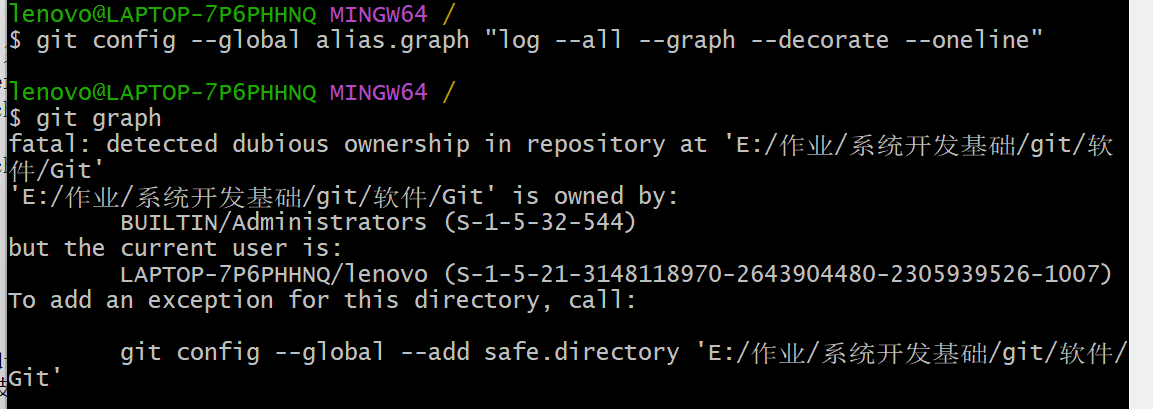
\includegraphics[width=\textwidth]{n3} % 确保文件名正确
    \caption{添加别名}
    \label{fig:remote-branch-check}
  \end{figure}
\end{itemize}









%1.2.16表格==================================================%


\subsubsection{设置全局 gitignore 文件以忽略特定于操作系统或特定于编辑器的文件 临时文件}
\begin{itemize}
  \item 命令展示
  \begin{verbatim}
   touch ~/.gitignore_global
git config --global core.excludesfile ~/.gitignore_global
# MacOS系统文件
.DS_Store

# Windows系统文件
Thumbs.db
ehthumbs.db
Desktop.ini

# 编辑器临时文件
*~
*.swp
*.swo
.idea/
.vscode/
*.bak

# Node.js
node_modules/


  \end{verbatim}

  \item 效果展示
  \begin{figure}[H]
    \centering
    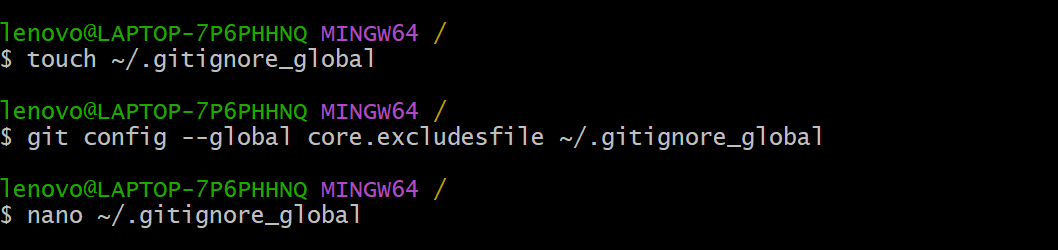
\includegraphics[width=\textwidth]{n5} % 确保文件名正确
    \caption{忽略特定于操作系统或特定于编辑器的文件 临时文件}
    \label{fig:remote-branch-check}
  \end{figure}
  \begin{figure}[H]
    \centering
    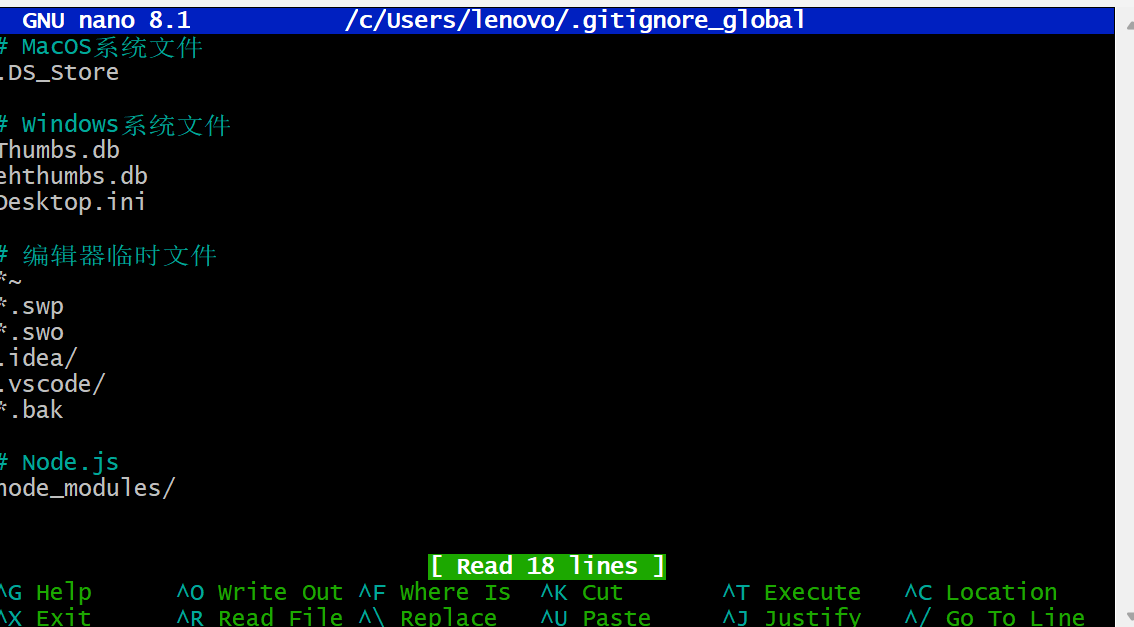
\includegraphics[width=\textwidth]{n6} % 确保文件名正确
    \caption{忽略特定于操作系统或特定于编辑器的文件 临时文件}
    \label{fig:remote-branch-check}
  \end{figure}
\end{itemize}




%1.2.16表格==================================================%


\subsubsection{为 GitHub 仓库提交一个有用的 Pull Request}
\begin{itemize}
  \item 命令展示
  \begin{verbatim}
git clone https://github.com/KeepingMoving/work1.git
cd work1
git checkout -b fix-typo
git add <modified-files>
git commit -m "Fix typo in README.md"
git push origin fix-typo



  \end{verbatim}

  \item 效果展示
  \begin{figure}[H]
    \centering
    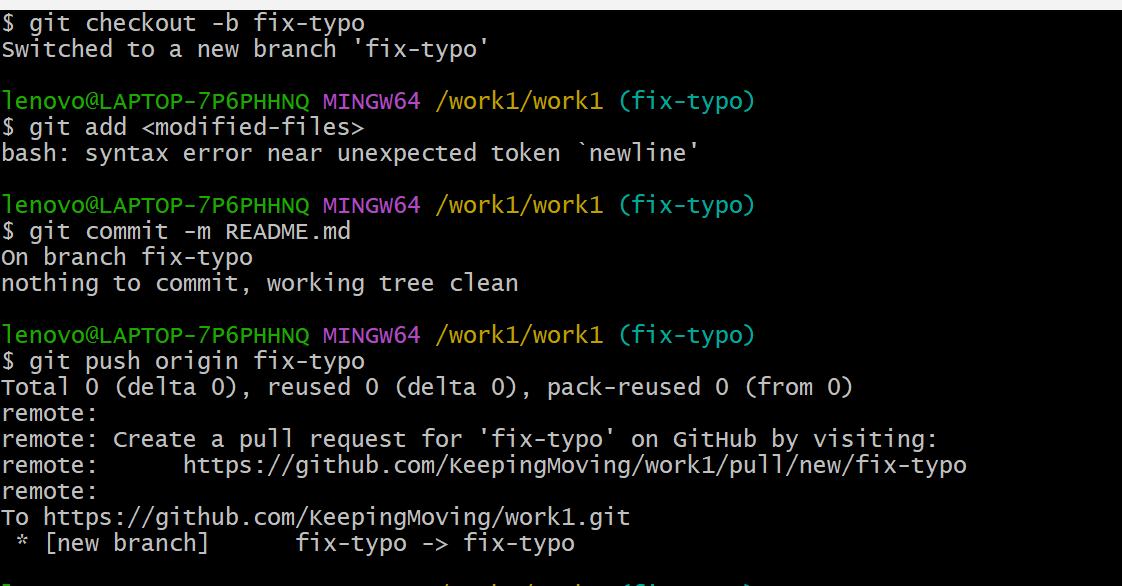
\includegraphics[width=\textwidth]{n10} % 确保文件名正确
    \caption{提交一个有用的 Pull Request}
    \label{fig:remote-branch-check}
  \end{figure}

\end{itemize}

%1.2.16表格==================================================%


\subsubsection{查看最后一个修改的人}
\begin{itemize}
  \item 命令展示
  \begin{verbatim}
git clone https://github.com/KeepingMoving/work1.git
cd work1
git log --graph --oneline --all
git log -1 -- README.md
git blame _config.yml
git show 09c08a2


  \end{verbatim}

  \item 效果展示
  \begin{figure}[H]
    \centering
    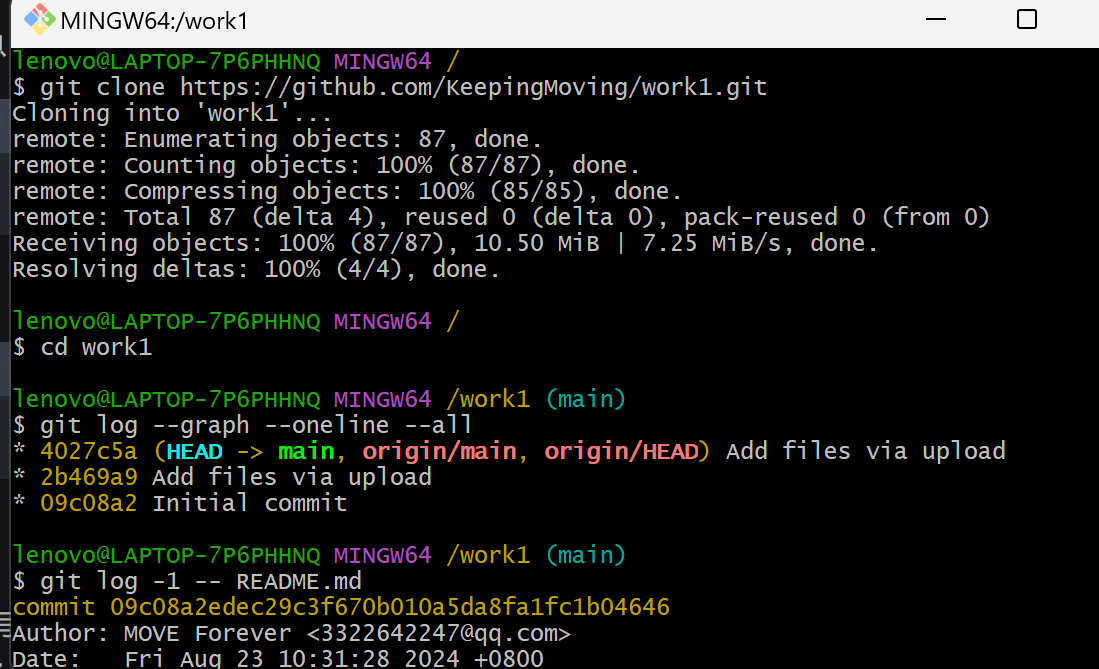
\includegraphics[width=\textwidth]{n7} % 确保文件名正确
    \caption{查看最后一个修改的人}
    \label{fig:remote-branch-check}
  \end{figure}
\begin{figure}[H]
    \centering
    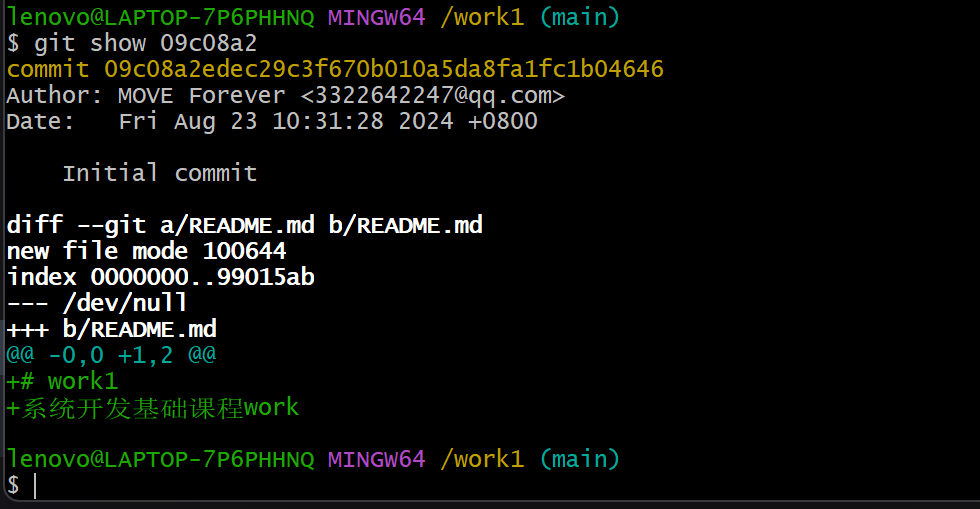
\includegraphics[width=\textwidth]{n8} % 确保文件名正确
    \caption{查看最后一个修改的人}
    \label{fig:remote-branch-check}
  \end{figure}

\end{itemize}


%1.2.16表格==================================================%
  \section{困难与解决方案}
  \subsection{LaTex}








\begin{itemize}
\item 问题:图片/表格插入跳行!!
\item 解决方案:通过float包解决

\item 问题:检查了好几个小时一直编译不通过!!!
\item 解决方案:因为aux文件没有完整输入,导致上次编译结束后aux文件的部分内容缺失。删除编译文件夹内.aux扩展名结尾的文件,重新用Latex命令进行编译,自动生成正确的aux文件,完成错误的修复。

\item 问题:编译成功但是目录没有显示
\item 解决方案:多编译两次
 \end{itemize}


\subsection{git}

\begin{itemize}
\item 问题:无法克隆
\item 解决方案:问题是由于没有配置信任的服务器HTTPS验证。默认,cURL被设为不信任任何CAs,就是说,它不信任任何服务器验证。执行下面命令就可以解决\\
git config --global http.sslVerify false


\item 问题: 切换分支报错:有文件未跟踪
\item 解决方案:尝试删除项目,然后从新安装,或者直接从现有的项目中把文件夹复制过来

\item 问题:git rm --cached 报错:recursively without -r
\item 解决方案:命令加上-f即可

\item 问题:同一个文件跟踪两次
\item 解决方案:使用git rm --cached来取消对重命名之前的文件跟踪
 \end{itemize}





  \section{心得体会}
\begin{itemize}
  \item LaTex对于数学公式,定理等编辑较为友好,大部分的数学公式都能通过命令展示,且排版较为整洁,但LaTex上手难度较高,且不如word这种可视化软件来得方便,通过代码来编写文档。\\
  \item git可以极大地简化了代码的管理和协同工作流程,但是仍是上手较难有阵痛期,各种配置也相对来说较为麻烦,单人使用不推荐,多人协作还不错。\\
  \item 通过本次学习我对LaTex和git有了一定的认识,LaTex和git都是十分有用的工具,山积则高,泽积则深,千里之行始于足下,希望在今后的学习中我能更加熟练地掌握LaTex和git这两个有用的工具。
\end{itemize}

  

  \section{github网址}
\href{https://github.com/KeepingMoving/work1.git}{GitHub仓库}
 










\end{document}